\documentclass{llncs}

\pagestyle{plain}


\usepackage[utf8]{inputenc}
\usepackage{amsmath,amssymb,latexsym}
\usepackage{url}
\usepackage{subfigure}
\usepackage{multirow}

\usepackage{tikz}
\usetikzlibrary{automata}
\usetikzlibrary{shapes.geometric}
\usetikzlibrary{intersections}
\tikzset{run/.style={minimum size=0.7cm,inner sep=2pt}}



\newcommand{\Nset}{\mathbb{N}}
\newcommand{\X}{\mathsf{X}}     \newcommand{\U}{{\,\uU\,}}      \newcommand{\uU}{\mathsf{U}}    \newcommand{\rR}{\mathsf{R}}    \newcommand{\R}{{\,\rR\,}}      \newcommand{\F}{\mathsf{F}}     \newcommand{\G}{\mathsf{G}}     \newcommand{\Fs}{{\F\!\s}}      \newcommand{\Gs}{{\G\s}}        \newcommand{\s}{_\mathsf{s}}    

\newcommand{\ttrue}{\mathtt{tt}}
\newcommand{\ffalse}{\mathtt{ff}}
\newcommand{\true}{\textrm{{\it tt}}}
\newcommand{\false}{\textrm{{\it ff}}}
\newcommand{\At}{{\it AP}}
\newcommand{\AP}{\mathit{A\hskip-0.1ex P}}
\newcommand{\LTL}{{\mathrm{LTL}}}
\newcommand{\suf}[1]{_{#1..}}

\newcommand{\mA}{\mathcal{A}}
\newcommand{\mB}{\mathcal{B}}
\newcommand{\mD}{\mathcal{D}}
\newcommand{\mG}{\mathcal{G}}
\newcommand{\mGR}{\mathcal{GR}}
\newcommand{\mR}{\mathcal{R}}
\newcommand{\mT}{\mathcal{T}}
\newcommand{\mI}{\mathcal{I}}
\newcommand{\mO}{\mathcal{O}}
\newcommand{\mZ}{\mathcal{Z}}
\newcommand{\A}{_{\mA}}			\newcommand{\T}{_{\mT}}			

\newcommand{\Ac}{\mathit{Ac}}
\newcommand{\Inf}{\mathit{Inf\!}}
\newcommand{\AC}{\mathrm{AC}}
\newcommand{\AT}[1]{\mathrm{AT}_{\!#1}}
\newcommand{\must}{\mathit{must}}
\newcommand{\may}{\mathit{may}}
\newcommand{\targets}{\mathit{targets}}

\def\exampleformula{\G(\F\s a \land \F\s b) \lor \G b}



\DeclareMathOperator*{\range}{{range}}
\DeclareMathOperator*{\dom}{{dom}}

\newcommand{\todo}[1]{\marginpar{\color{red}#1}}
\newcommand{\kickoff}[1]{\textcolor{blue}{#1}}
\usepackage{xcolor}
\newcommand{\added}[1]{\colorlet{foo}{.}\color{black!70!red!40!green}#1\color{foo}}



\makeatletter

\pgfkeys{/pgf/.cd,
  rectangle corner radius/.initial=3pt
}
\newif\ifpgf@rectanglewrc@donecorner@
\def\pgf@rectanglewithroundedcorners@docorner#1#2#3#4{\edef\pgf@marshal{\noexpand\pgfintersectionofpaths
      {\noexpand\pgfpathmoveto{\noexpand\pgfpoint{\the\pgf@xa}{\the\pgf@ya}}\noexpand\pgfpathlineto{\noexpand\pgfpoint{\the\pgf@x}{\the\pgf@y}}}{\noexpand\pgfpathmoveto{\noexpand\pgfpointadd
          {\noexpand\pgfpoint{\the\pgf@xc}{\the\pgf@yc}}{\noexpand\pgfpoint{#1}{#2}}}\noexpand\pgfpatharc{#3}{#4}{\cornerradius}}}\pgf@process{\pgf@marshal\pgfpointintersectionsolution{1}}\pgf@process{\pgftransforminvert\pgfpointtransformed{}}\pgf@rectanglewrc@donecorner@true
}
\pgfdeclareshape{rectangle with rounded corners}
{
  \inheritsavedanchors[from=rectangle] \inheritanchor[from=rectangle]{north}
  \inheritanchor[from=rectangle]{north west}
  \inheritanchor[from=rectangle]{north east}
  \inheritanchor[from=rectangle]{center}
  \inheritanchor[from=rectangle]{west}
  \inheritanchor[from=rectangle]{east}
  \inheritanchor[from=rectangle]{mid}
  \inheritanchor[from=rectangle]{mid west}
  \inheritanchor[from=rectangle]{mid east}
  \inheritanchor[from=rectangle]{base}
  \inheritanchor[from=rectangle]{base west}
  \inheritanchor[from=rectangle]{base east}
  \inheritanchor[from=rectangle]{south}
  \inheritanchor[from=rectangle]{south west}
  \inheritanchor[from=rectangle]{south east}

  \savedmacro\cornerradius{\edef\cornerradius{\pgfkeysvalueof{/pgf/rectangle corner radius}}}

  \backgroundpath{\northeast\advance\pgf@y-\cornerradius\relax
    \pgfpathmoveto{}\pgfpatharc{0}{90}{\cornerradius}\northeast\pgf@ya=\pgf@y\southwest\advance\pgf@x\cornerradius\relax\pgf@y=\pgf@ya
    \pgfpathlineto{}\pgfpatharc{90}{180}{\cornerradius}\southwest\advance\pgf@y\cornerradius\relax
    \pgfpathlineto{}\pgfpatharc{180}{270}{\cornerradius}\northeast\pgf@xa=\pgf@x\advance\pgf@xa-\cornerradius\southwest\pgf@x=\pgf@xa
    \pgfpathlineto{}\pgfpatharc{270}{360}{\cornerradius}\northeast\advance\pgf@y-\cornerradius\relax
    \pgfpathlineto{}}

  \anchor{before north east}{\northeast\advance\pgf@y-\cornerradius}
  \anchor{after north east}{\northeast\advance\pgf@x-\cornerradius}
  \anchor{before north west}{\southwest\pgf@xa=\pgf@x\advance\pgf@xa\cornerradius
    \northeast\pgf@x=\pgf@xa}
  \anchor{after north west}{\northeast\pgf@ya=\pgf@y\advance\pgf@ya-\cornerradius
    \southwest\pgf@y=\pgf@ya}
  \anchor{before south west}{\southwest\advance\pgf@y\cornerradius}
  \anchor{after south west}{\southwest\advance\pgf@x\cornerradius}
  \anchor{before south east}{\northeast\pgf@xa=\pgf@x\advance\pgf@xa-\cornerradius
    \southwest\pgf@x=\pgf@xa}
  \anchor{after south east}{\southwest\pgf@ya=\pgf@y\advance\pgf@ya\cornerradius
    \northeast\pgf@y=\pgf@ya}

  \anchorborder{\pgf@xb=\pgf@x \pgf@yb=\pgf@y \southwest \pgf@xa=\pgf@x \pgf@ya=\pgf@y \northeast \advance\pgf@x by-\pgf@xa \advance\pgf@y by-\pgf@ya \pgf@xc=.5\pgf@x \pgf@yc=.5\pgf@y \advance\pgf@xa by\pgf@xc \advance\pgf@ya by\pgf@yc \edef\pgf@marshal{\noexpand\pgfpointborderrectangle
      {\noexpand\pgfqpoint{\the\pgf@xb}{\the\pgf@yb}}
      {\noexpand\pgfqpoint{\the\pgf@xc}{\the\pgf@yc}}}\pgf@process{\pgf@marshal}\advance\pgf@x by\pgf@xa \advance\pgf@y by\pgf@ya \pgfextract@process\borderpoint{}\pgf@rectanglewrc@donecorner@false
\southwest\pgf@xc=\pgf@x\pgf@yc=\pgf@y
    \advance\pgf@xc\cornerradius\relax\advance\pgf@yc\cornerradius\relax 
    \borderpoint
    \ifdim\pgf@x<\pgf@xc\relax\ifdim\pgf@y<\pgf@yc\relax
      \pgf@rectanglewithroundedcorners@docorner{-\cornerradius}{0pt}{180}{270}\fi\fi
\ifpgf@rectanglewrc@donecorner@\else
      \southwest\pgf@yc=\pgf@y\relax\northeast\pgf@xc=\pgf@x\relax
      \advance\pgf@xc-\cornerradius\relax\advance\pgf@yc\cornerradius\relax
      \borderpoint
      \ifdim\pgf@x>\pgf@xc\relax\ifdim\pgf@y<\pgf@yc\relax
       \pgf@rectanglewithroundedcorners@docorner{0pt}{-\cornerradius}{270}{360}\fi\fi
    \fi
\ifpgf@rectanglewrc@donecorner@\else
      \northeast\pgf@xc=\pgf@x\relax\pgf@yc=\pgf@y\relax
      \advance\pgf@xc-\cornerradius\relax\advance\pgf@yc-\cornerradius\relax
      \borderpoint
      \ifdim\pgf@x>\pgf@xc\relax\ifdim\pgf@y>\pgf@yc\relax
       \pgf@rectanglewithroundedcorners@docorner{\cornerradius}{0pt}{0}{90}\fi\fi
    \fi
\ifpgf@rectanglewrc@donecorner@\else
      \northeast\pgf@yc=\pgf@y\relax\southwest\pgf@xc=\pgf@x\relax
      \advance\pgf@xc\cornerradius\relax\advance\pgf@yc-\cornerradius\relax
      \borderpoint
      \ifdim\pgf@x<\pgf@xc\relax\ifdim\pgf@y>\pgf@yc\relax
       \pgf@rectanglewithroundedcorners@docorner{0pt}{\cornerradius}{90}{180}\fi\fi
    \fi
  }
}

\makeatother



\begin{document}
\frontmatter



\title{Effective Translation of LTL to Deterministic Rabin Automata: Beyond
  the (F,G)-Fragment\thanks{This is a full version of the paper accepted to
    ATVA 2013.}}
\author{Tom\'{a}\v{s} Babiak \and Franti\v{s}ek Blahoudek \and Mojm\'{i}r
  K\v{r}et\'{i}nsk\'{y} \and Jan Strej\v{c}ek}
\institute{Faculty of Informatics, Masaryk University, Brno, Czech Republic\\
\email{\{xbabiak,\,xblahoud,\,kretinsky,\,strejcek\}@fi.muni.cz}}



\maketitle




\begin{abstract}
  Some applications of linear temporal logic (LTL) require to translate
  formulae of the logic to deterministic -automata. There are
  currently two translators producing deterministic automata:
  \texttt{ltl2dstar} working for the whole LTL and Rabinizer applicable to
  LTL() which is the LTL fragment using only modalities  and .  We
  present a new translation to deterministic Rabin automata via alternating
  automata and deterministic transition-based generalized Rabin
  automata. Our translation applies to a fragment that is strictly larger
  than LTL(). Experimental results show that our algorithm can produce
  significantly smaller automata compared to Rabinizer and
  \texttt{ltl2dstar}, especially for more complex LTL formulae.
\end{abstract}	



\section{Introduction}

\emph{Linear temporal logic (LTL)} is a popular formalism for specification
of behavioral system properties with major applications in the area of model
checking~\cite{CGP99,BK08}. More precisely, LTL is typically used as a
human-oriented front-end formalism as LTL formulae are succinct and easy to
write and understand. Model checking algorithms usually work with an
-automaton representing all behaviors violating a given
specification formula rather than with the LTL formula directly. Hence,
specifications written in the form of LTL formulae are negated and
translated to equivalent -automata~\cite{VardiW86}. There has been a
lot of attention devoted to translation of LTL to \emph{nondeterministic
  B\"uchi automata (NBA)}, see for example~\cite{Cou99,DGV99,SB00,GO01} and
the research in this direction still continues~\cite{DL11,BKRS12,BBDL13}.  However,
there are algorithms that need specifications given by \emph{deterministic}
-automata, for example, those for LTL model checking of
probabilistic systems~\cite{Vardi85,CY95,BK08} and those for synthesis of
reactive modules for LTL specifications~\cite{Church62,PnueliR89}, for a
recent survey see \cite{Kupferman12}.
As \emph{deterministic B\"uchi automata (DBA)} cannot express all the
properties expressible in LTL, one has to choose deterministic automata with
different acceptance condition.


There are basically two approaches to translation of LTL to
deterministic -automata. The first one translates LTL to NBA
and then it employs Safra's construction~\cite{Saf88} (or some of its
variants or alternatives like~\cite{Pit07,Sch09}) to transform the NBA into
a deterministic automaton. This approach is represented by the
tool \texttt{ltl2dstar}~\cite{Kle} which uses an improved Safra's
construction~\cite{KB06,KB07} usually in connection with LTL to NBA
translator LTL2BA~\cite{GO01}. The main advantage of this approach is its
universality: as LTL2BA can translate any LTL formula into an NBA and the
Safra's construction can transform any NBA to a \emph{deterministic Rabin
  automaton (DRA)}, \texttt{ltl2dstar} works for the whole LTL. The main
disadvantage is also connected with the universality: the determinization
step does not employ the fact that the NBA represents only an LTL definable
property. One can easily observe that \texttt{ltl2dstar} produces
unnecessarily large automata, especially for formulae with more fairness
subformulae.

The second approach is to avoid Safra's construction.
As probabilistic model-checkers deal with linear arithmetic, 
they do not profit 
from symbolically represented deterministic automata
of~\cite{PPS06,MorgensternS08}.
A few translations of some simple LTL fragments to DBA have been
suggested, for example \cite{AT04}.  
Recently, a translation of
a~significantly larger LTL fragment to DRA has been introduced
in~\cite{KE12} and subsequently implemented in the tool
Rabinizer~\cite{GKE12}. The algorithm builds a~\emph{generalized
  deterministic Rabin automata (GDRA)} directly from a formula. A~DRA is
then produced by a degeneralization procedure. Rabinizer often produces
smaller automata than \texttt{ltl2dstar}. The main disadvantage is that
it works for LTL() only, i.e.~the LTL fragment containing only
temporal operators \emph{eventually} () and \emph{always}
(). Authors of the translation claim that it can be extended to
a~fragment containing also the operator \emph{next} ().

In this paper, we present another Safraless translation of an LTL
fragment to DRA. 
The translation is influenced by the successful LTL
to NBA translation algorithm LTL2BA~\cite{GO01}
and it proceeds in the following three steps:
\begin{enumerate}
\item A given LTL formula  is translated into a \emph{very weak
    alternating co-B\"uchi automaton (VWAA)}  as described
  in~\cite{GO01}. If  is an LTL() formula, i.e.~any
  formula which makes use of , , and their strict variants  and
   as the only temporal operators,
then  satisfies an additional structural condition. We call such
  automata \emph{may/must alternating automata (MMAA)}.
\item The MMAA  is translated into a \emph{transition-based
    generalized deterministic Rabin automaton (TGDRA)} .  The
  construction of generalized Rabin pairs of  is inspired
  by~\cite{KE12}.
\item Finally,  is degeneralized into a (state-based) DRA .  \end{enumerate}

In summary, our contributions are as follows.  First, note that the
fragment LTL() is strictly more expressive than
LTL(). Moreover, it can be shown that our translation works for a
fragment even larger than LTL() but still smaller than the
whole LTL. 
Second, the translation has a slightly better theoretical bound on the
size of produced automata comparing to \texttt{ltl2dstar}, but the same
bound as Rabinizer. Experimental results show that, for small formulae,
our translation typically produces automata of a smaller or equal size
as the other two translators.  However, for parametrized formulae, it
often produces automata that are significantly smaller. Third, we note
that our TGDRA are much smaller than the (state-based) GDRA
of~Rabinizer~\cite{GKE12}. We conjecture that algorithms for model checking of
probabilistic system, e.g.~those in PRISM~\cite{KNP11}, can be adapted
to work with TGDRA as they are adapted to work with GDRA~\cite{CGK13}.














\section{Preliminaries}\label{sec:prelim}
This section recalls the notion of linear temporal logic (LTL)~\cite{Pnu77} 
and describes the -automata used in the following.



\subsubsection{Linear Temporal Logic (LTL)}

The syntax of LTL is defined by

where  stands for \emph{true},  ranges over a countable set 
of \emph{atomic propositions},  and  are temporal operators called
\emph{next} and \emph{until}, respectively. An \emph{alphabet} is a finite
set , where  is a finite subset of . An
\emph{-word} (or simply a \emph{word}) over  is an infinite
sequence of letters . By  we
denote the suffix .


We inductively define when a word  \emph{satisfies} a formula ,
written , as follows.
\begin{center}
\begin{tabbing}
  \hspace*{1em} \= \\
  \>  \hspace*{2.7em} \= iff~ \= \\
  \>  \> iff \> \\
  \>  \> iff \>
   or \\
  \>  \> iff \>
   and \\
  \>  \> iff \> \\
  \>  \> iff \>
      and
     
\end{tabbing}
\end{center}

Given an alphabet , a formula  defines the language
. We 
write  instead of , where
 denotes the set of atomic propositions occurring in the
formula .

We define derived unary temporal operators \emph{eventually}
(), \emph{always} (), \emph{strict eventually} (), and
\emph{strict always} () by the
following equivalences: ,
, , and
.

LTL() denotes the LTL fragment consisting of formulae built with
temporal operators  and  only.  The fragment build with temporal
operators , ,  and  is denoted by LTL() as
 and  can be seen as abbreviations for
 and , respectively.  Note
that LTL() is strictly more expressive than LTL() as
formulae  and  cannot be equivalently expressed in
LTL(). 

An LTL formula is in \emph{positive normal form} if no operator occurs in
the scope of any negation.  Each LTL() formula can be transformed
to this form using De Morgan's laws for  and  and the
equivalences , ,
, and . We say that
a formula is \emph{temporal} if its topmost operator is neither conjunction,
nor disjunction (note that  and  are also temporal formulae).



\subsubsection{Deterministic Rabin Automata and Their Generalization}



A \emph{semiautomaton} is a tuple , where  is
a finite set of \emph{states},  is an alphabet,  is the
\emph{initial state}, and  is a
deterministic \emph{transition relation}, i.e.~for each state  and
each , there is at most one state  such that
. A triple  is called a
\emph{transition} from  to  labelled by , or an
-transition of  leading to .  In illustrations, all
transitions with the same source state and the same target state are usually
depicted by a single edge labelled by a propositional formula  over
 representing the corresponding transition labels (e.g.~given
, the formula  represents labels
).

A \emph{run} of a semiautomaton  over a word  is an infinite sequence  of transitions such that
. By  (resp.~) we denote the set of
transitions (resp.~states) occurring infinitely often in . For each
word , a semiautomaton has at most one run over 
denoted by .

A \emph{deterministic Rabin automaton} (DRA) is a tuple
, where  is a
semiautomaton and  is a finite set
of \emph{Rabin pairs}.
Runs of  are runs of the semiautomaton.  A run  \emph{satisfies}
a Rabin pair  if  and
.  A run is \emph{accepting} if it
satisfies some Rabin pair of . The language of  is the set
 of all words  such that  is
accepting.



A \emph{transition-based generalized deterministic Rabin automaton} (TGDRA)
is a tuple , where
 is a semiautomaton and  is a finite set of \emph{generalized Rabin
  pairs}.  
Runs of  are runs of the semiautomaton.  A run 
\emph{satisfies} a generalized Rabin pair  if  and, for each
, .  A run is \emph{accepting}
if it satisfies some generalized Rabin pair of .  The language
of  is the set  of all words  such that
 is accepting.

A generalization of DRA called \emph{generalized deterministic Rabin
  automata} (GDRA) has been considered in~\cite{KE12,GKE12}. The accepting
condition of GDRA is a positive Boolean combination (in disjunctive normal
form) of Rabin pairs. A run  is accepting if  satisfies this
condition.








\subsubsection{Very Weak Alternating Automata and Their Subclass}
\label{def:MMAA}

A \emph{very weak alternating co-B\"{u}chi automaton} (VWAA) 
is a tuple , where  is a finite set of
\emph{states}, subsets  are called \emph{configurations},
 is an \emph{alphabet},  is an \emph{alternating transition relation},  is a
non-empty set of \emph{initial configurations},  is a set of
\emph{co-B\"{u}chi accepting states}, and there exists a partial order on
 such that, for every transition , all the states
of  are lower or equal to .

A triple  is called a transition from  to 
labelled by , or an -transition of .  We say that  is
the \emph{source state} and  the \emph{target configuration} of the
transition.  A transition is \emph{looping} if the target configuration
contains the source state, i.e.~.  A transition is called a
\emph{selfloop} if its target configuration contains the source state only,
i.e.~.



\begin{figure}[!t]
  \centering
  \subfigure[]{\label{fig:alt}
    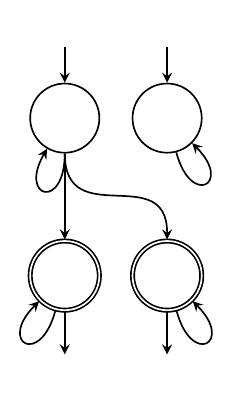
\begin{tikzpicture}[auto,initial where=above,initial text=,semithick,>=stealth]


\node[state,initial]   (s0) at (0,2){};
      \node[state,accepting](s1) at (0,0){};
      \node[state,accepting](s2) at (1.3,0){};
      \node[state,initial]   (s3) at (1.3,2){};
      \node[] (placeholder) at (0.65,-1) {\strut};

      \path[->] (s0) edge node [right,pos=0.65] {} (s1) 
      (s0) edge [out=-90,in=90,looseness=1.5] node {} (s2)
      (s0) edge [looseness=8,out=-90,in=-120,overlay] node [] {} (s0);
      \path[->] (s3) edge [looseness=8,out=-75,in=-45,overlay] node [right,pos=.63] {} (s3);
      \path[->] (s1) edge [looseness=8,out=-105,in=-135,overlay] node [left,pos=.63] {} (s1)
      (s1) edge [] node [right] {} +(0,-1)	 	 
      (s2) edge [looseness=8,out=-75,in=-45,overlay] node [right,pos=.63] {} (s2)
      (s2) edge [] node [left] {} +(0,-1);
    \end{tikzpicture}
  }~
  \subfigure[]{\label{fig:vwaarun}
    \def\xbase{0.7} 
    \def\yG{3}
    \def\yFa{2}
    \def\yFb{1}
    \def\yGb{0}
    \def\yl{\yG+0.4}
    \def\ylast{\yGb}
    \def\length{8}

    \begin{tikzpicture}[inner sep=0pt,>=stealth,
      dot/.style={fill=black,circle,minimum size=5pt},xscale=0.85]
\node[state,run] at (0,\yG) {};
      \node[state,run,accepting] at (0,\yFa) {};
      \node[state,run,accepting] at (0,\yFb) {};
      \node[state,run] at (0,\yGb) {};
      \node[] (placeholder) at (0.65,-.5) {\strut};

\node at (0.5+\xbase, \yG+0.5) {};
      \node at (1.5+\xbase, \yG+0.5) {};
      \node at (2.5+\xbase, \yG+0.5) {};
      \node at (3.5+\xbase, \yG+0.5) {};
      \node at (4.5+\xbase, \yG+0.5) {};
      \node at (5.5+\xbase, \yG+0.5) {};
      \node at (6.5+\xbase, \yG+0.5) {};
      \node at (7.5+\xbase, \yG+0.5) {};


\foreach \x in {0,...,\length} \node[dot] (G\x) at (\xbase+\x,\yG) {};
      \foreach \x in {1,...,\length} \node[dot] (Fa\x) at (\xbase+\x,\yFa) {};
      \foreach \x in {1,...,\length} \node[dot] (Fb\x) at (\xbase+\x,\yFb) {};

\foreach \x in {0,...,7} {
	\node[dot] (G\x+1) at (\xbase+\x+1,\yG) {};
	\node[dot] (Fa\x+1) at (\xbase+\x+1,\yFa) {};
	\node[dot] (Fb\x+1) at (\xbase+\x+1,\yFb) {};	
	\path[->] (G\x) edge (G\x+1);
	\path[->] (G\x) edge (Fa\x+1);
	\path[->] (G\x) edge (Fb\x+1);
      }

\path[->] (Fb1) edge (Fb2)
                (Fa1) edge (Fa2)
                (Fa2) edge (Fa3)
                (Fb4) edge (Fb5)	
                (Fb5) edge (Fb6)
                (Fa5) edge (Fa6)	
                (Fa6) edge (Fa7);
                
\path[->] (Fb2) edge +(0.3,-0.3)
      		    (Fa3) edge +(0.3,-0.3)
      		    (Fb3) edge +(0.3,-0.3)
      		    (Fa4) edge +(0.3,-0.3)
				(Fb7) edge +(0.3,-0.3)
				(Fa7) edge +(0.3,-0.3)
				(Fb6) edge +(0.3,-0.3);
\node at (\xbase+\length+0.5,\yFb+0.5) {};
		  
\foreach \x in {0,...,\length} {
        \draw[dotted] (\xbase+\x,\ylast-0.3) to (\xbase+\x,\yG+0.3);
        \node at (\xbase+\x,\yG+0.3) {\tiny{\x}};
      }

\foreach \x in {0,...,7} \node at (\xbase+\x+0.5,\ylast-0.5) {\small{}};
    \end{tikzpicture}
  }
  \caption{\subref{fig:alt} A VWAA (and also
    MMAA) corresponding to formula , where . \subref{fig:vwaarun} An accepting run of the automaton
over .}
\end{figure}



Figure~\ref{fig:alt} shows a VWAA that accepts the
language described by the formula .
Transitions are depicted by branching edges.  If a target configuration
is empty, the corresponding edge leads to an empty space.  We often depict all
transitions with the same source state and the same target configuration by
a single edge (as for semiautomata).  Each initial configuration is
represented by a possibly branching unlabelled edge leading from an empty
space to the states of the configuration.  Co-B\"{u}chi accepting states are
double circled.



A \emph{multitransition}  with a label  is a set of transitions
with the same label and such that the source states of the transitions are
pairwise different.  A \emph{source configuration} of , denoted by
, is the set of source states of transitions in .  A
\emph{target configuration} of , denoted by , is the union of
target configurations of transitions in .  We define a
\emph{multitransition relation}  as 



A \emph{run}  of a VWAA  over a word  is an infinite sequence  of multitransitions of
 such that  is an initial configuration of  and, for
each ,  is labelled by  and . 

A run can be represented as a directed acyclic graph (DAG).  For example,
the DAG of Figure~\ref{fig:vwaarun} represents a run of the VWAA of
Figure~\ref{fig:alt}.  The dotted lines divide the DAG into segments
corresponding to multitransitions.  Each transition of a multitransition is
represented by edges leading across the corresponding segment from the
starting state to states of the target configuration. As our alternating
automata are very weak, we can order the states in a way that all edges
in any DAG go only to the same or a lower row.

An accepting run corresponds to a DAG where each branch contains only
finitely many states from .  Formally, the run  is \emph{accepting}
if it has no suffix where, for some co-B\"{u}chi accepting state ,
each multitransition contains a looping transition from . The language of
 is the set .  By  we denote the set of states that
occur in  for infinitely many indices .





\begin{definition}\label{def:mmaa}
  A \emph{may/must alternating automaton} (MMAA)
  is a VWAA where each state fits into one of the following three
  categories:
  \begin{enumerate}
  \item \emph{May-states} -- states with a selfloop for each
    .  A run that enters such a state \emph{may} wait in
    the state for an arbitrary number of steps.
  \item \emph{Must-states} -- every transition of a must-state is looping. A
    run that enters such a state can never leave it. In other words, the run
    \emph{must} stay there.
  \item \emph{Loopless states} -- states that have no looping transitions
    and no predecessors. They can appear only in initial configurations (or
    they are unreachable).
  \end{enumerate}
\end{definition}

The automaton of Figure~\ref{fig:alt} is an MMAA with must-states
 and may-states .

We always assume that the set  of an MMAA coincides with the set of all may-states of the automaton.  This
assumption is justified by the following observations:
\begin{itemize}
\item There are no looping transitions of loopless states. Hence,
  removing all loopless states from  has no effect on acceptance of
  any run.
\item All transitions leading from must-states are looping. Hence, if a
  run contains a must-state that is in , then the run is
  non-accepting.  Removing all must-states in  together with their
  adjacent transitions from an MMAA has no effect on its accepting runs.
\item Every may-state has selfloops for all . If such a
  state is not in , we can always apply these selfloops without violating
  acceptance of any run. We can also remove these states from all the target
  configurations of all transitions of an MMAA without affecting its
  language.
\end{itemize}





\section{Translation of LTL() to MMAA}\label{sec:corr}

We present the standard translation of LTL to VWAA~\cite{GO01} restricted to
the fragment LTL().  In this section, we treat the transition
relation  of a VWAA as a function
, where  means
.  Further, we consider  and  to be
subformulae of  and , respectively.  This is justified by
equivalences  and .  Recall
that a formula is called \emph{temporal} if its topmost operator is neither
conjunction, nor disjunction (note that  and  are also temporal
formulae).

Let  be an  formula in positive normal form.  An
equivalent VWAA is constructed as , where
\begin{itemize}
\item  is the set of temporal subformulae of ,
\item ,
\item  is defined as 
  
  
\item  where  is defined
  as 
  
\item  is the set of all subformulae of the form  in .
\end{itemize}

Using the partial order ``is a subformula of'' on states, one can easily
prove that  is a VWAA.  Moreover, all the states of the form
 are must-states and all the states of the form  are may-states.
States of other forms are loopless and they are unreachable unless they
appear in . Hence, the constructed automaton is also an MMAA.
Figure~\ref{fig:alt} shows an MMAA produced by the translation of formula
.



In fact, MMAA and LTL() are expressively equivalent.  The reverse
translation can be found in Appendix~\ref{sec:mmaa2ltl}.



\section{Translation of MMAA to TGDRA}
\label{sec:MMAA2DRA}
In this section we present a translation of an MMAA  with multitransition relation  into an
equivalent TGDRA . At first we build a semiautomaton  by a double
powerset construction (performing dealternation and determinization of the
MMAA). Then we describe the transition based generalized Rabin acceptance
condition  of .



\subsection{Semiautomaton }
\label{sec:ts}
The idea of our seminautomaton construction is straightforward: a run
 of the semiautomaton  tracks all runs of  over .
More precisely, the state of  reached after reading a finite input
consists of all possible configurations in which  can be after reading
the same input.  Hence, states of the semiautomaton are sets of
configurations of  and we call them \emph{macrostates}.  We use
 to denote states of  ( stands for an accepting
state of ),  to denote configurations of , and
 to denote macro\-states of .  Further, we use
 to denote the transitions of ,  to
denote multitransitions of , and  to denote the
transitions of , which are called \emph{macrotransitions} hereafter.


Formally, we define the \emph{semiautomaton } 
for  as follows:
\begin{itemize}
\item  is the set \emph{macrostates}, restricted to
  those reachable from the initial macrostate  by ,
\item  iff , i.e.~for each  and
  , there is a single macrotransition
  , where  consists of target
  configurations of all -multitransitions leading from
  configurations in , and
\item  is the \emph{initial macrostate}.
\end{itemize}




Figure~\ref{fig:ts} depicts the semiautomaton  for the MMAA of
Figure~\ref{fig:alt}. Each row in a macrostate represents one configuration.























		  


    
















		  


    




\begin{figure}[t]
  \centering
    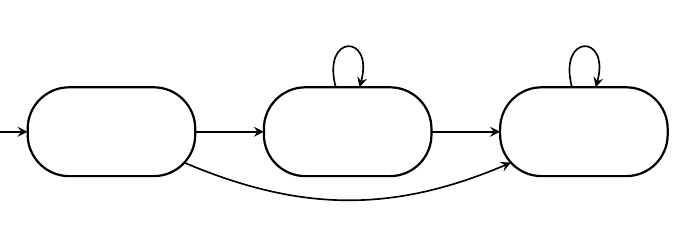
\begin{tikzpicture}[auto,initial where=left,initial text=,
      semithick,>=stealth,trim left=(init.west),trim right=(gp.east)]
\tikzstyle{state}=[shape=rectangle with rounded corners,
        rectangle corner radius=15pt,thick,draw,
        minimum width=2.1cm, minimum height=1.1cm,inner sep=2pt,align=center]
\node[state,initial] (init) at (0,0) { \\ };
      \node[state] (gpgb) at (3,0) { \\ };
      \node[state] (gp) at (6,0) {};
\path[->]
      (init) edge [] node [above] {} (gpgb)
      (init) edge [bend right=23] node [below,overlay] {} (gp)	
      (gpgb) edge [loop above,looseness=6] node [above] {} (gpgb)
      (gpgb) edge [] node [above] {} (gp)
      (gp) edge [loop above,looseness=6] node [above] {} (gp);
\end{tikzpicture}
    
\caption{The semiautomaton  for the MMAA of Figure \ref{fig:alt}.}
  \label{fig:ts}
\end{figure}





\subsection{Acceptance Condition  of the TGDRA }
For any subset ,  denotes the set of must-states
of . An MMAA run  is \emph{bounded by}  iff  and .  For example, the run of
Figure~\ref{fig:vwaarun} is bounded by the set .

For any fixed , we define the set  of
\emph{allowed configurations} of  and the set  of \emph{allowed macrotransitions} of  as follows:

\footnotetext{A definition of  with  would
  be more intuitive, but less effective.}  Clearly, a run  of  is
bounded by  if and only if  has a suffix containing only
configurations of . Let  be a run over  with such a
suffix. As the semiautomaton  tracks all runs of  over a given
input, the run  of  `covers' also . Hence, 
has a suffix where, for each macrotransition , there
exist configurations  and 
satisfying . In other words,  has a
suffix containing only macrotransitions of .  This observation is
summarized by the following lemma.
\begin{lemma}\label{lem:aux}
  If  has a run over  bounded by , then the run  of
   contains a suffix of macrotransitions of .
\end{lemma}
In fact, the other direction can be proved as well: if  contains
a suffix of macrotransitions of , then  has a run over 
bounded by .

For each , we also define the set  as the set of all
macrotransitions in  such that  contains a non-looping
transition of  with the same label and with the target configuration not
leaving :


Using the sets  and , we define one generalized Rabin pair
 for each subset of states :


\begin{lemma}\label{lem:ag}
If there is an accepting run  of  over  then the run 
 of  satisfies  for .
\end{lemma}
\begin{proof}
  As  is bounded by , Lemma~\ref{lem:aux} implies that 
  has a suffix  of macrotransitions of . Thus
  .

  As  and  is accepting, for each ,  includes infinitely many multitransitions  where
   and  contains a non-looping transition
   satisfying  and . Hence,
  the corresponding macrotransitions  that are also in the mentioned
  suffix  of  are elements of .
  Therefore,  for each  and  satisfies .\qed
\end{proof}

\begin{lemma}\label{lem:ga}
If a run  of  satisfies  then there is
an \emph{accepting} run of  over  bounded by .
\end{lemma}
\begin{proof}
  Let  be a run of  satisfying ,
  i.e.~ has a suffix of macrotransitions of  and
   contains infinitely many macrotransitions of  for
  each .  Let  be the first
  macrotransition of the suffix.  The definition of  implies that
  there is a configuration .  The construction of
   guarantees that there exists a sequence of multitransitions of 
  leading to the configuration . More precisely, there is a sequence
   such that  is an initial configuration of
  ,  is labelled by  for each ,
   for each , and .  We
  show that this sequence is in fact a prefix of an accepting run of 
  over  bounded by . 

  We inductively define a multitransition sequence 
  completing this run.  The definition uses the suffix
   of .  Let us assume that  and that
   is a configuration of .  We define  to
  contain one -transition of  for each .  Thus
  we get .  As , there exists a
  multitransition  labelled by  such that both source and target
  configurations of  are in .  For each must-state
  ,  contains the same transition leading from 
  as contained in .  For may-states , we have two
  cases.  If ,  contains a non-looping transition
  leading from  to some states in .  The existence of such a
  transition follows from the definition of .  For the remaining
  may-states,  uses selfloops.
Formally, , where

One can easily check that  and we continue by building
.  

To sum up, the constructed run is bounded by .  Moreover,  contains
no looping transition of  whenever . As the run
 is accepting,  holds infinitely often for each
. The constructed run of  over  is thus accepting.\qed
\end{proof}

The previous two lemmata give us the following theorem.
\begin{theorem}
The TGDRA  describes the same
language as .
\end{theorem}














\section{Translation of TGDRA to DRA}
This section presents a variant of the standard degeneralization procedure.  
At first we illustrate the idea on a TGDRA
 with one
generalized Rabin pair. Recall
that a run is accepting if it has a suffix not using macrotransitions of 
and using macrotransitions of each  infinitely often.

An equivalent DRA  consists of  copies of . The copies are
called \emph{levels}.  We start at the level .  Intuitively, being at a
level  for  means that we are waiting for a transition from
.  Whenever a transition of  appears, we move to the level .  A
transition  gets us from a level  to the maximal level  such that  for each . The levels  and 
have the same transitions (including target levels) as the level . A run
of  is accepting if and only if the corresponding run of  visits
the level  only finitely often and it visits the level  infinitely
often.





In the general case, we track the levels for all generalized Rabin pairs
simultaneously. Given a TGDRA
, we construct an equivalent DRA as , where
\begin{itemize}
\item ,
\item  
iff  and for each  it holds

\item ,
\item , and
\item .
\end{itemize}



\section{Complexity}

This section discusses the upper bounds of the individual steps of our
translation and compares the overall complexity to the complexity of the
other translations.

Given a formula  of LTL(), we produce an MMAA with
at most  states, where  is the length of .  Then we build the
TGDRA  with at most  states and at most  generalized
Rabin pairs.  To obtain the DRA , we multiply the state space by at
most  for each generalized Rabin pair .  The value of 
is bounded by . Altogether, we can derive an upper bound on the number of
states of the resulting DRA as

which is the same bound as in \cite{KE12}, but lower than  of \texttt{ltl2dstar}.  It is worth mentioning that the number of
states of our TGDRA is bounded by  while the number of
states of the GDRA produced by Rabinizer is bounded by
. 



\section{Simplifications and Translation Improvements}
\label{sec:simplifications}

An important aspect of our translation process is simplification of all
intermediate results leading to smaller resulting DRA.

We simplify input formulae by reduction rules of LTL3BA,
see~\cite{BKRS12} for more details. Additionally, we rewrite the
subformulae of the form  and  to equivalent
formulae  and  respectively. This preference of
strict temporal operators often yields smaller resulting automata.

Alternating automata are simplified in the same way as in LTL2BA: removing
unreachable states, merging equivalent states, and removing redundant
transitions, see~\cite{GO01} for details.

We improve the translation of an MMAA  to a TGDRA  in order to
reduce the number of generalized Rabin pairs of .  One can observe
that, for any accepting run  of ,  contains
only states reachable from some must-state.  Hence, in the construction of
acceptance condition of  we can consider only subsets  of states
of  of this form.  Further, we omit a subset  if, for each
accepting run over  bounded by , there is also an accepting run
over  bounded by some .  The formal description of
subsets  considered in the construction of the TGDRA  is described
in Appendix~\ref{app:Zset}.

If a run  of an MMAA satisfies  for
some , then  for all  and the run is accepting.
We use this observation to improve the construction of the semiautomaton
 of the TGDRA : if a macrostate  contains the empty
configuration, we remove all other configurations from .


After we build the TGDRA, we simplify its acceptance condition in three
ways (similar optimizations are also performed by Rabinizer).
\begin{enumerate}
\item We remove some generalized Rabin pairs 
  that cannot be satisfied by any run, in particular when  or  for some .
\item We remove  if there is some  such that .
\item If the fact that a run  satisfies the pair  implies that
   satisfies also some other pair , we remove .
\end{enumerate}

Finally, we simplify the state spaces of both TGDRA and DRA such that we
iteratively merge the equivalent states. Two states of a DRA  are
equivalent if they belong to the same sets of the acceptance condition of
 and, for each , their -transitions lead to the same
state. Two states of a TGDRA  are equivalent if, for each ,
their -transitions lead to the same state and belong to the same
sets of the acceptance condition of . Moreover, if the initial state of
 or  has no selfloop, we check its equivalence to another state
regardless of the acceptance condition (note that a membership in acceptance
condition sets is irrelevant for states or transitions that are passed at
most once by any run).



Of course, we consider only the reachable state space at every step.



\section{Beyond LTL(,) Fragment: May/Must in the Limit}
\label{sec:limmmaa}

The Section \ref{sec:MMAA2DRA} shows a translation of MMAA into TGDRA.  In
fact, our translation can be used for a larger class of very weak
alternating automata called \emph{may/must in the limit automata} (limMMAA).
A VWAA  is a limMMAA if  contains only must-states, states without
looping transitions, and co-B\"{u}chi accepting states (not exclusively
may-states), and each state reachable from a must-state is either a must- 
or a may-state. Note that each accepting run of a limMMAA has a suffix that
contains either only empty configurations, or configurations consisting of
must-states and may-states reachable from must-states. Hence, the MMAA to
TGDRA translation produces correct results also for limMMAA under an
additional
condition: generalized Rabin pairs  are constructed only for sets
 that contain only must-states and may-states reachable from them.

We can obtain limMMAA by the LTL to VWAA translation of \cite{GO01} when it
is applied to an LTL fragment defined as

where  ranges over LTL(,). Note that this fragment is
strictly more expressive than LTL(,).





\section{Experimental Results}
\label{sec:experiments}
We have made an experimental implementation of our translation (referred to
as \emph{LTL3DRA}). The translation of LTL to alternating automata is taken
from LTL3BA~\cite{BKRS12}.  We compare the automata produced
by LTL3DRA to those produced by Rabinizer and \texttt{ltl2dstar}. All the
experiments are run on a Linux laptop (2.4GHz Intel Core i7, 8GB of RAM)
with a timeout set to 5 minutes.

Tables given below (i) compare the sizes of the DRA produced by all the
tools and (ii) show the number of states of the generalized automata
produced by LTL3DRA and Rabinizer. Note that LTL3DRA uses TGDRA
whereas Rabinizer uses (state-based) GDRA,
hence the numbers of their states cannot be
directly compared. The sizes of DRA are written as , where  is the
number of states and  is the number of Rabin pairs.  For each formula,
the size of the smallest DRA (measured by the number of states and, in the
case of equality, by the number of Rabin pairs) is printed in bold.



\begin{table}[t!]
\centering
\setlength{\tabcolsep}{3pt}
\small
\begin{tabular}{|c|c||rc|rr|r|}
\hline
\multicolumn{2}{ |c|| }{\multirow{2}{*}{Formula} } &
  \multicolumn{2}{ |c| }{LTL3DRA} & 
  \multicolumn{2}{ c| }{Rabinizer} &
  \multicolumn{1}{ |c| }{\texttt{ltl2dstar}}
  \\ \cline{3-7}
\multicolumn{2}{ |c|| }{} &
\multicolumn{2}{|r|}{\scriptsize DRA~~~TGDRA} & \multicolumn{2}{|r|}{\scriptsize DRA~~GDRA} & \multicolumn{1}{ |c|  }{\scriptsize DRA}   \\ \cline{1-7}
\multicolumn{2}{ |c|| }{}& \textbf{3(2)}& 2 & 4(2) & 5~ & 4(1) \\
\multicolumn{2}{ |c|| }{}& \textbf{8(3)}& 1 & \textbf{8(3)} & 8~ & \textbf{8(3)} \\
\multicolumn{2}{ |c|| }{}& \textbf{2(1)}& 2 & \textbf{2(1)} & 2~ & \textbf{2(1)} \\
\multicolumn{2}{ |c|| }{}& \textbf{2(1)}& 1 & \textbf{2(1)} & 4~ & \textbf{2(1)} \\
\multicolumn{2}{ |c|| }{}& \textbf{2(1)}& 1 & 2(2) & 2~ & \textbf{2(1)} \\
\multicolumn{2}{ |c|| }{}& \textbf{2(1)}& 2 & \textbf{2(1)} & 8~ & 3(1) \\
\multicolumn{2}{ |c|| }{}& \textbf{3(2)}& 2 & 4(2) & 9~ & 4(1) \\
\multicolumn{2}{ |c|| }{}& \textbf{3(2)}& 3 & \textbf{3(2)} & 3~ & 4(2) \\
\multicolumn{2}{ |c|| }{}& \textbf{3(2)}& 2 & 4(2) & 11~ & 4(1) \\
\multicolumn{2}{ |c|| }{}& \textbf{4(2)}& 1 & \textbf{4(2)} & 4~ & \textbf{4(2)} \\
\multicolumn{2}{ |c|| }{}& \textbf{3(1)}& 1 & \textbf{3(1)} & 8~ & 7(2) \\
\multicolumn{2}{ |c|| }{}& \textbf{1(0)}& 1 & \textbf{1(0)} & 1~ & \textbf{1(0)} \\
\multicolumn{2}{ |c|| }{}& \textbf{3(1)}& 1 & \textbf{3(1)} & 4~ & \textbf{3(1)} \\
\multicolumn{2}{ |c|| }{}& \textbf{4(2)}& 1 & \textbf{4(2)} & 4~ & 5(2) \\
\multicolumn{2}{ |c|| }{}& \textbf{2(1)}& 1 & \textbf{2(1)} & 2~ & \textbf{2(1)} \\
\multicolumn{2}{ |c|| }{}& \textbf{3(1)}& 1 & \textbf{3(1)} & 4~ & 5(1) \\
\multicolumn{2}{ |c|| }{}& \textbf{4(1)}& 4 & \textbf{4(1)} & 4~ & \textbf{4(1)} \\
\multicolumn{2}{ |c|| }{}& \textbf{12(3)}& 4 & 18(4) & 18~ & 13(3) \\
\multicolumn{2}{ |c|| }{}& \textbf{4(2)}& 4 & 6(3) & 18~ & 14(4) \\
\multicolumn{2}{ |c|| }{}& \textbf{5(2)}& 4 & \textbf{5(2)} & 18~ & 7(1) \\
\multicolumn{2}{ |c|| }{}& \textbf{5(2)}& 4 & \textbf{5(2)} & 18~ & 7(2) \\
\multicolumn{2}{ |c|| }{}& \textbf{4(3)}& 1 & \textbf{4(3)} & 4~ & 14(4) \\
\multicolumn{2}{ |c|| }{}& \textbf{4(3)}& 1 & \textbf{4(3)} & 4~ & 145(9) \\
\multicolumn{2}{ |c|| }{}& \textbf{4(3)}& 1 & \textbf{4(3)} & 4~ & 145(9) \\
\hline
\multirow{4}{*}{}
&&\textbf{4(2)}& 1 & \textbf{4(2)} & 4~ & \textbf{4(2)} \\
&&\textbf{18(4)}& 1 & 20(4) & 16~ & 11324(8) \\
&&\textbf{166(8)}& 1 & 470(8) & 64~ & \multicolumn{1}{|c|}{timeout}\\
&&\textbf{7408(16)}& 1 & \multicolumn{2}{|c|}{timeout} & \multicolumn{1}{|c|}{timeout}\\
\hline
\multirow{5}{*}{}
&&\textbf{4(2)}& 1 & \textbf{4(2)} & 4~ & \textbf{4(2)} \\
&&\textbf{10(4)}& 1 & 11(4) & 8~ & 572(7) \\
&&\textbf{36(6)}& 1 & 52(6) & 16~ & 290046(13) \\
&&\textbf{178(9)}& 1 & 1288(9) & 32~ & \multicolumn{1}{|c|}{timeout}\\
&&\textbf{1430(14)}& 1 & \multicolumn{2}{|c|}{timeout} & \multicolumn{1}{|c|}{timeout}\\
&&\textbf{20337(22)}& 1 & \multicolumn{2}{|c|}{timeout} & \multicolumn{1}{|c|}{timeout}\\
\hline
\multicolumn{3}{c}{}&\multicolumn{1}{c}{~~~~~~~~~}&\multicolumn{1}{c}{}&\multicolumn{1}{c}{~~~~~~}
\end{tabular}
\smallskip
\caption{The benchmark from \cite{GKE12} extended by one parametric formula.} 
\label{tab:ATVA}
\end{table}



Table \ref{tab:ATVA} shows the results on formulae from \cite{GKE12}
extended with another parametric formula. For the two parametric formulae,
we give all the parameter values  for which at least one tool finished
before timeout. For all formulae in the table, our experimental
implementation generates automata of the same or smaller size as the others.
Especially in the case of parametric formulae, the automata produced by
LTL3DRA are considerably smaller. We also note that the TGDRA constructed
for the formulae are typically very small.


Table~\ref{tab:SPEC} shows the results on formulae from \textsc{Spec
  Patterns}~\cite{DAC99} (available
online\footnote{\url{http://patterns.projects.cis.ksu.edu/documentation/patterns/ltl.shtml}}).
We only take formulae LTL3DRA is able to work with, i.e.~the formulae of the
LTL fragment defined in Section~\ref{sec:limmmaa}.  The fragment covers 27
out of 55 formulae listed on the web page.  The dash sign in Rabinizer's
column means that Rabinizer cannot handle the corresponding formula as it is
not from the LTL() fragment.  For most of the formulae in the table,
LTL3DRA produces the smallest DRA. In the remaining cases, the DRA produced
by our translation is only slightly bigger than the smallest one.  The table
also illustrates that LTL3DRA handles many (pseudo)realistic formulae not
included in LTL().  
Four more parametric benchmarks are provided in Appendix~\ref{sec:moreexp}.




\begin{table}[t!]
\centering
\begin{tabular}{|c||r c|rc|r|c|c||rc|rc|r|}
\cline{1-6}\cline{8-13}
\multicolumn{1}{ |c|| }{\multirow{2}{*}{} } &
  \multicolumn{2}{ |c| }{LTL3DRA} & 
  \multicolumn{2}{ c| }{Rabinizer} &
  \multicolumn{1}{ |c| }{\texttt{ltl2dstar}}&
 \multicolumn{1}{c}{~~} &
\multicolumn{1}{ |c|| }{\multirow{2}{*}{} } &
  \multicolumn{2}{ |c| }{LTL3DRA} & 
  \multicolumn{2}{ c| }{Rabinizer} &
  \multicolumn{1}{ |c| }{\texttt{ltl2dstar}}
 \\  \cline{2-6}\cline{9-13}
\multicolumn{1}{ |c||  }{} &
\multicolumn{2}{|c|}{\scriptsize DRA~~TGDRA} & \multicolumn{2}{|c|}{\scriptsize DRA~~GDRA} & \multicolumn{1}{ |c|  }{\scriptsize DRA} &
\multicolumn{1}{ |c|  }{} & \multicolumn{1}{ |c||  }{} &
\multicolumn{2}{|c|}{\scriptsize DRA~~TGDRA} & \multicolumn{2}{|c|}{\scriptsize DRA~~GDRA} & \multicolumn{1}{ |c|  }{\scriptsize DRA}\\  
\cline{1-6}\cline{8-13}
 & \textbf{4(2)}& 4 & \multicolumn{2}{|c|}{---}  & 5(2)~~~ & &  & \textbf{4(2)}& 4 & \multicolumn{2}{|c|}{---}  & 5(2)~~~~\\  
 & ~~4(2)& 3 & ~~4(2) & 5 & \textbf{4(1)}~~~ & &  & ~~6(3)& 3 & ~~8(3) & 14 & \textbf{5(1)}~~~~\\ 
 & \textbf{4(2)}& 3 & \multicolumn{2}{|c|}{---}  & \textbf{4(2)} ~~~&&  & \textbf{4(2)}& 4 & \multicolumn{2}{|c|}{---}  & 6(2)~~~~\\  
 & \textbf{3(2)}& 3 & \textbf{3(2)} & 5 & 4(2) ~~~&&  & \textbf{5(2)}& 5 & \multicolumn{2}{|c|}{---}  & 7(2)~~~~\\  
 & \textbf{6(2)}& 6 & \multicolumn{2}{|c|}{---}  & 10(3) ~~~&&  & \textbf{5(2)}& 5 & \multicolumn{2}{|c|}{---}  & 7(3)~~~~\\ 
 & \textbf{8(2)}& 8 & \multicolumn{2}{|c|}{---}  & 9(2) ~~~&&   & 6(3)& 4 & \multicolumn{2}{|c|}{---}  & \textbf{6(2)}~~~~\\ 
 & \textbf{7(3)}& 7 & \multicolumn{2}{|c|}{---}  & 11(3) ~~~&&   & \textbf{6(2)}& 6 & \multicolumn{2}{|c|}{---}  & 8(3)~~~~\\ 
 & \textbf{4(2)}& 4 & \multicolumn{2}{|c|}{---}  & 5(2) ~~~&&   & 7(4)& 5 & \multicolumn{2}{|c|}{---}  & \textbf{6(3)}~~~~\\  
 & 4(2)& 3 & 4(2) & 5 & \textbf{4(1)} ~~~&&   & \textbf{21(3)}& 7 & \multicolumn{2}{|c|}{---}  & 45(3)~~~~\\  
 & \textbf{4(2)}& 3 & \multicolumn{2}{|c|}{---}  & \textbf{4(2)} ~~~&&   & \textbf{12(2)}& 12~ & \multicolumn{2}{|c|}{---}  & 17(2)~~~~\\  
 & \textbf{4(2)}& 4 & \multicolumn{2}{|c|}{---}  & 5(2) ~~~&&   & \textbf{15(3)}& 5 & \multicolumn{2}{|c|}{---}  & 20(2)~~~~\\  
 & \textbf{5(3)}& 4 & \multicolumn{2}{|c|}{---}  & \textbf{5(3)} ~~~&&   & 7(2)& 7 & \multicolumn{2}{|c|}{---} & \textbf{6(2)}~~~~\\  
 & \textbf{3(2)}& 2 & 4(2) & 5 & 4(1) ~~~&&   & \textbf{14(3)}& 6 & \multicolumn{2}{|c|}{---}  & 24(2)~~~~\\  
\cline{1-6}
\multicolumn{7}{c|}{}& & 7(2)& 7 & \multicolumn{2}{|c|}{---}  & \textbf{6(2)}~~~~\\  
\cline{8-13}
\end{tabular}
\caption{The benchmark with selected formulae from \textsc{Spec
    Patterns}.  denotes the -th formula on the web page.}
\label{tab:SPEC}
\end{table}





\section{Conclusion}\label{sec:concl}
We present another Safraless translation of an LTL fragment to deterministic
Rabin automata (DRA).  Our translation employs a new class of \emph{may/must
  alternating automata}.  We prove that the class is expressively equivalent
to the LTL() fragment.  Experimental results show that our
translation typically produces DRA of a smaller or equal size as the other
two translators of LTL (i.e.~Rabinizer and \texttt{ltl2dstar}) and it
sometimes produces automata that are significantly smaller.





\bibliographystyle{abbrv}
\bibliography{atva}

\newpage
\appendix



\section{Translation of MMAA to LTL()}\label{sec:mmaa2ltl}
We can assume that may-states have no looping transitions except
selfloops. Indeed, any application of a looping transition that is not a
selfloop can be always replaced by an application of a selfloop with the
same label. This change is safe as it cannot transform an accepting run into
a non-accepting one.

Let  be an MMAA. For any , we 
define  to be a formula satisfied exactly by the words starting 
with :
 
Now we inductively define a formula  for each .  The
formula  is satisfied by any word for which there is an
accepting run of  starting in the configuration .  Admissibility of
the inductive definition follows from the fact that  is a very weak
automaton, i.e.~there is a partial order on  such that transitions of a
state  can lead only to  or lower states.

Note that the conjunction of an empty set of conjuncts is  while
the disjunction of an empty set of disjuncts is . It is easy to see
that each temporal operator  in  is in front of  or .
If we replace all occurrences of  by  and all occurrences of
 by ,
we always get formulae of LTL().

Finally, we define the formula  equivalent to the whole
automaton  as


Hence, we have shown that the following theorem holds.
\begin{theorem}
  For each MMAA  with an alphabet of the form , we can
  construct an LTL() formula  such that
  .
\end{theorem}



\section{Bounding Sets}\label{app:Zset}

Let  be an MMAA or a limMMAA.  Here
we show how to compute the set  of configurations
for which the generalized Rabin pairs  of the
corresponding TGDRA are constructed.  If  is an accepting run of , then
 is a subset of states reachable from must-states.  Further,
for each  there is an accepting run  over  such that,
for each , either , or  uses a single
non-looping transition of  (infinitely often) and the selfloop for~.
We say that these runs are \emph{modest}.

The function  recursively computes, for a given
state , the sets of states that can potentially be reached from  (not
necessary as one configuration) infinitely often by a modest run visiting
 infinitely often. If  is a may-state, a modest run uses only one of
the non-looping transitions of  and possibly also the selfloop of .
If  is a must-state, a modest run can use an arbitrary combination of
transitions of . Formally,  is defined as
3ex]
   \{\{s\}\} \otimes \bigcup_{C \subseteq {\targets(s)}}  \mathbf{z}(\bigcup\limits_{c 
   \in C} c)      & \text{if } s \in \must(S)\text{,}
  \end{cases}

W_1 \otimes W_2 = \textstyle \bigcup_{\substack{c_1 \in W_1 \\
    c_2 \in W_2}} \{c_1 \cup c_2\}\text{,}

\targets(s) = \left\{ c \in 2^{S\smallsetminus\{s\}} \mid (s, \alpha,c \cup
  \{s\}) \in \delta\A, \alpha \in \Sigma\right\}\text{,}

\mathbf{z}(c) = \textstyle \bigotimes_{s \in c} z(s)
\qquad\textrm{and}\qquad
\mathbf{z}(\emptyset) = \{\emptyset\}.

  y(s) = &\begin{cases}
   \bigcup_{\substack{(s,\alpha,c) \in \delta\A, \\ s \notin c}} \mathbf{y}(c) & 
   \text{if } s \notin \must(S) \
where  is an auxiliary function defined for each configuration
as


Finally, the set  of configurations  for which we construct the
generalized Rabin pairs  of the corresponding TGDRA is defined as
.
Note that the states that are not successors of any must-state are not
included in any element of the set .



\section{More Experimental Results}\label{sec:moreexp}


Table~\ref{tab:app} provides experimental results for four parametric
formulae, namely  of~\cite{GO01}, its negation
,  of~\cite{GH06}, and
 of~\cite{GH06}. Note that
 and  are outside the fragment LTL(,).


In all the cases but one (), LTL3DRA generates DRA of the same size as
the other tools or smaller.  Finally, LTL3DRA runs slower than
\texttt{ltl2dstar} on , while it is the fastest on the other three
formulae.  We list all instances of the formulae for which at least one of
the tools produces a DRA before timeout.



\begin{table}[b]
\centering
\begin{tabular}{|c||r@{\quad}r@{\quad}|r@{\quad}r@{\quad}|r@{\quad}|}
\hline
\multicolumn{1}{ |c|| }{\multirow{2}{*}{Formula} } &
  \multicolumn{2}{ |c }{LTL3DRA} & 
  \multicolumn{2}{ |c| }{Rabinizer} &
  \multicolumn{1}{ |c| }{\texttt{~ltl2dstar~}}
  \\ \cline{2-6}
\multicolumn{1}{ |c||  }{} &
\multicolumn{2}{|r|}{\scriptsize DRA~~~TGDRA} & \multicolumn{2}{|r|}{\scriptsize DRA~~GDRA} & \multicolumn{1}{ |c|  }{\scriptsize DRA}  \\ \cline{1-6}
\hline  & \textbf{3(1)}& 2 & \textbf{3(1)} & 10 & 4(1) \\
 & \textbf{4(1)}& 2 & 5(1) & 20 & 8(1) \\
 & \textbf{5(1)}& 2 & 7(1) & 40 & 12(1) \\
 & \textbf{6(1)}& 2 & 9(1) & 80 & 16(1) \\
 & \textbf{7(1)}& 2 & 11(1) & 160 & 20(1) \\
 & \textbf{8(1)}& 2 & 13(1) & 320 & 24(1) \\
 & \textbf{9(1)}& 2 & \multicolumn{2}{|c|}{timeout} & 28(1) \\
 & \textbf{10(1)}& 2 & \multicolumn{2}{|c|}{timeout} & 32(1) \\
 & \textbf{11(1)}& 2 & \multicolumn{2}{|c|}{timeout} & 36(1) \\
 & \textbf{12(1)}& 2 & \multicolumn{2}{|c|}{timeout} & \multicolumn{1}{|c|}{timeout}\\
 & \textbf{13(1)}& 2 & \multicolumn{2}{|c|}{timeout} & \multicolumn{1}{|c|}{timeout}\\
 & \textbf{14(1)}& 2 & \multicolumn{2}{|c|}{timeout} & \multicolumn{1}{|c|}{timeout}\\
\hline
 & \textbf{6(3)}& 2 & 8(3) & 10 & 7(2) \\
 & \textbf{12(4)}& 2 & 16(4) & 20 & 13(3) \\
 & \textbf{24(5)}& 2 & 32(5) & 40 & 25(4) \\
 & \textbf{48(6)}& 2 & 64(6) & 80 & 49(5) \\
 & \textbf{96(7)}& 2 & 128(7) & 160 & 97(6) \\
 & \textbf{192(8)}& 2 & \quad 256(8) & 320 & 193(7) \\
 & \textbf{384(9)}& 2 & \multicolumn{2}{|c|}{timeout}  & 385(8) \\
 & \textbf{768(10)}& 2 & \multicolumn{2}{|c|}{timeout}  & 769(9) \\
 & \textbf{1536(11)}& 2 & \multicolumn{2}{|c|}{timeout}  & 1537(10) \\
 & \textbf{3072(12)}& 2 & \multicolumn{2}{|c|}{timeout}  & 3073(11) \\
 & \quad\textbf{6144(13)}& 2 & \multicolumn{2}{|c|}{timeout}  & \multicolumn{1}{|c|}{timeout}\\
\hline
 & \textbf{3(1)}& 3 & \multicolumn{2}{|c|}{---} & \textbf{3(1)} \\
 & \textbf{5(1)}& 5 & \multicolumn{2}{|c|}{---} & \textbf{5(1)} \\
 & \textbf{9(1)}& 9 & \multicolumn{2}{|c|}{---} & \textbf{9(1)} \\
 & 24(1)& 24 & \multicolumn{2}{|c|}{---} & \textbf{17(1)} \\
 & \textbf{68(1)}& 68 & \multicolumn{2}{|c|}{---} & \multicolumn{1}{|c|}{timeout}\\
 & \textbf{212(1)}& 212 & \multicolumn{2}{|c|}{---} & \multicolumn{1}{|c|}{timeout}\\
 & \textbf{719(1)}& 719 & \multicolumn{2}{|c|}{---} & \multicolumn{1}{|c|}{timeout}\\
\hline
 & \textbf{3(1)}& 3 & \multicolumn{2}{|c|}{---} & \textbf{3(1)} \\
 & \textbf{4(1)}& 4 & \multicolumn{2}{|c|}{---} & \textbf{4(1)} \\
 & \textbf{5(1)}& 5 & \multicolumn{2}{|c|}{---} & \textbf{5(1)} \\
 & \textbf{6(1)}& 6 & \multicolumn{2}{|c|}{---} & \textbf{6(1)} \\
 & \textbf{7(1)}& 7 & \multicolumn{2}{|c|}{---} & \textbf{7(1)} \\
 & \textbf{8(1)}& 8 & \multicolumn{2}{|c|}{---} & \textbf{8(1)} \\
 & \textbf{9(1)}& 9 & \multicolumn{2}{|c|}{---} & \textbf{9(1)} \\
 & \textbf{10(1)}& 10 & \multicolumn{2}{|c|}{---} & \textbf{10(1)} \\
 & \textbf{11(1)}& 11 & \multicolumn{2}{|c|}{---} & \textbf{11(1)} \\
 & \textbf{12(1)}& 12 & \multicolumn{2}{|c|}{---} & \textbf{12(1)} \\
 & \textbf{13(1)}& 13 & \multicolumn{2}{|c|}{---} & \textbf{13(1)} \\
 & \multicolumn{2}{c|}{timeout} & \multicolumn{2}{|c|}{---} & \textbf{14(1)} \\
\hline
\end{tabular}
\smallskip
\caption{More parametric benchmarks.} 
\label{tab:app}
\end{table}







\end{document}
